\chapter{Methodology}
\label{ch:methodology}
This chapter contains the overarching research strategy and defines the methods used in the research.
\section{Research Model}
\label{sec:researchmodel}
This section describes the research steps. The detailed information on how these steps are operationalised are part of, \cref{sec:researchapproach}. \cref{fig:research-model} gives an overview on the steps that are taken to answer the main research question, \cref{sec:introresearchquestion}.
	\begin{figure}[H]
		\centering
		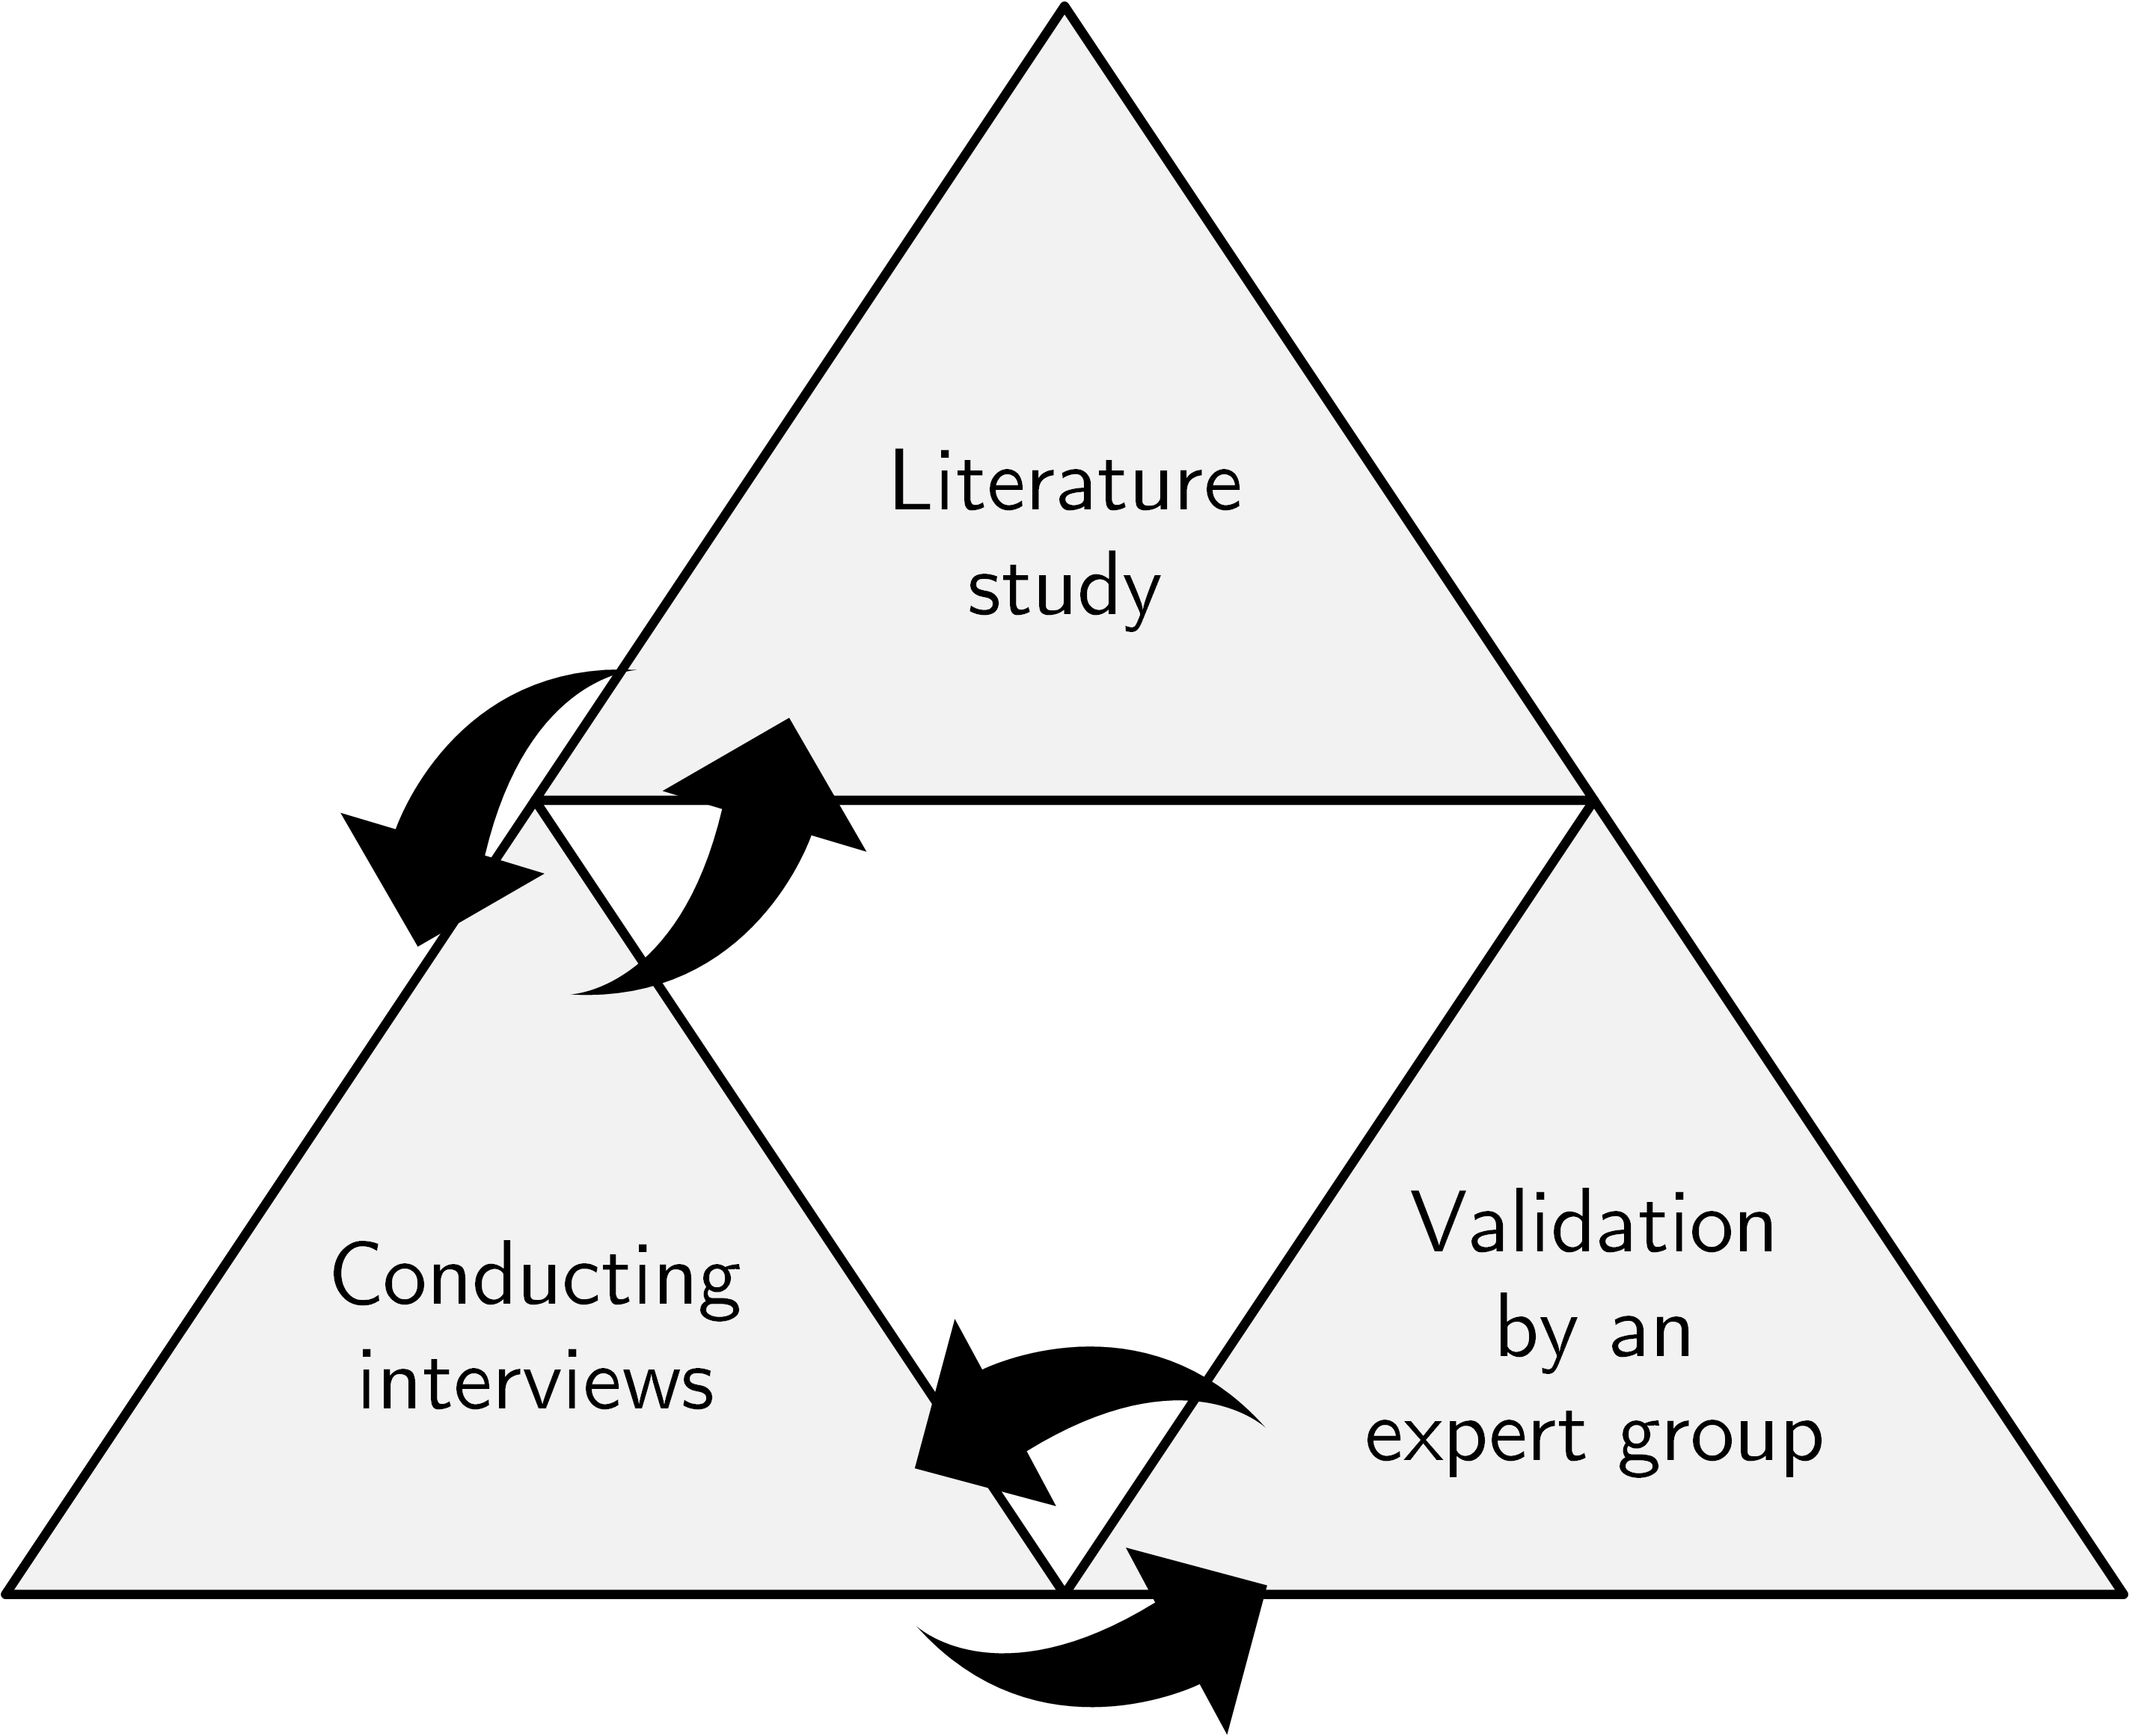
\includegraphics[width=14cm]{images/researchmodel}
		\caption[Research Model]{Research Model}
		\label{fig:research-model}
	\end{figure}
To answer the sub-questions and the main research question literature research has a central part in the approach. The research starts with a literature study on the concepts of systems, the \gls{ps}, \gls{antifragile}, and \acrfull{ea}. The goal of this step is to define the concepts and search for attributes that can possible be a success factor. The output with be analysed and possible success factors are determined. The outcome of this analysis will be validated by interviews. The interviews are analysed to validate the possible success factors and possible new success factors. The outcome will be validated by an Expert Group. After the validation by the expert group the final analysis will take place before conclusions are taken and a discussion on the outcome will take place.
\section{Research approach}
\label{sec:researchapproach}
This section elaborates on the detailed approach of the research.
\subsection{Literature study}
\label{sub:literaturestudy}
The literature study will answer most of the sub-questions as stated in \cref{sec:introresearchquestion}. The questions ''What is the literature saying about the \gls{ps}?'', ''What is the literature saying about \gls{antifragile}?'', ''What are the possible success factors of \gls{antifragile}?'', ''What is the literature saying about \acrlong{ea}?'' and ''What are possible success factors of \acrlong{ea}?'' will be answered. The answers will be split up into two chapters. These chapters are \cref{ch:theoreticalbackground} and \cref{ch:attributes}. For the literature research, two primary methods are used. The first method is (forward and backwards) snowballing of already acquired and found literature. In the literature administration, it is easy to recognize snowballing by using the column \textit{Found at}, see \cref{sub:tbresearchexecution}. The second method is the use of online scientific libraries.
\begin{figure}[H]
	\centering
	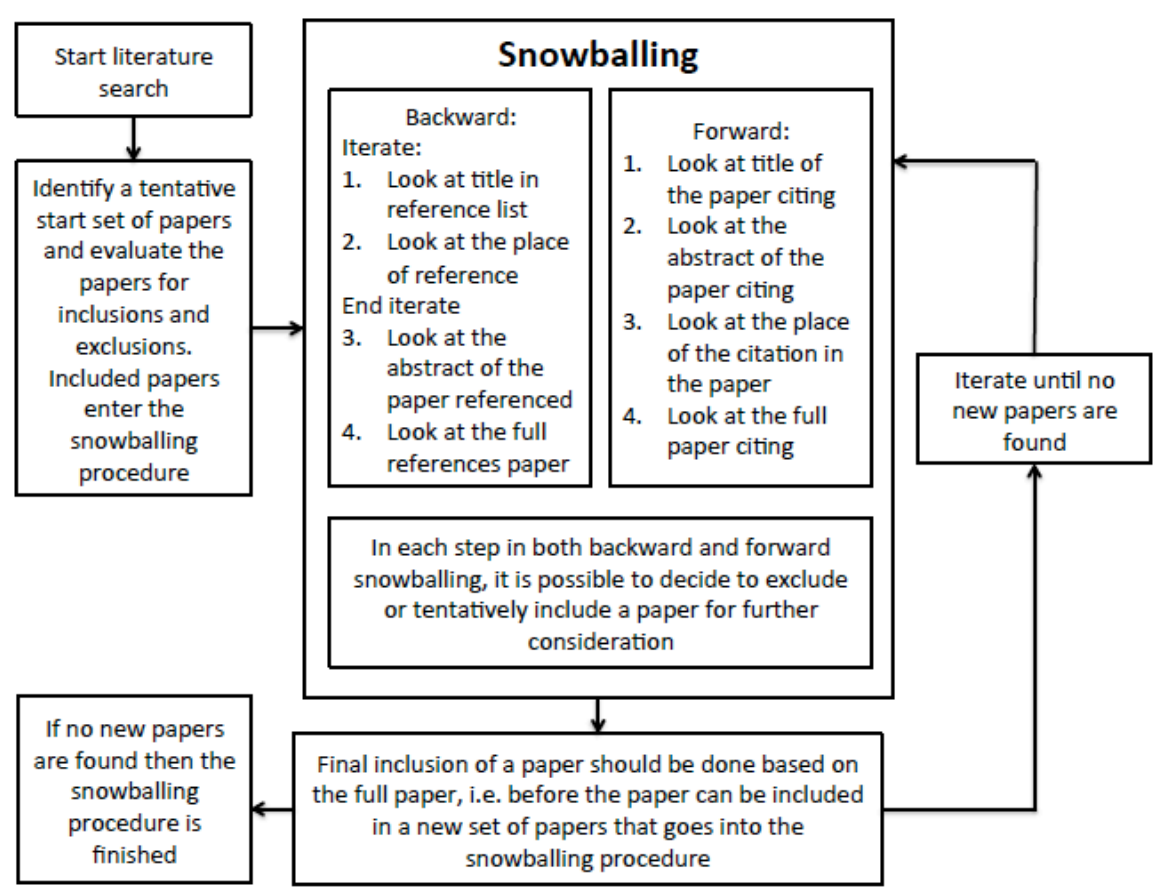
\includegraphics[width=0.6\linewidth]{images/snowball}
	\caption[Snowballing literature]{Snowballing literature \parencite{Wohlin2014}}
	\label{fig:snowball}
\end{figure}
For finding relevant literature online scientific libraries are used. The online scientific libraries are Web of Science, Research Gate, Google Scholar, and Semantic Scholar. The full concept name is used and the known abbreviations of the concept (e.g. Enterprise Architecture and EA). Literature is only accepted if the literature complies with quality attributes. These attributes are accuracy, authority, objectivity, currency, and coverage\footnote{\url{https://libguides.library.cityu.edu.hk/litreview/evaluating-sources/}}. All found literature is administrated for replicability, independence, precision, accessibility, and reusability. Section \ref{sub:tbresearchexecution} describes how literature registration and administration is executed.
\subsubsection{System}
\label{subsub:system}
For the literature study on system two primary sources are used. The first is that of \textcite{Ackoff1973} with the title \citetitle{Ackoff1973} and the second is that of \textcite{Gharajedaghi2011} with the title of \citetitle{Gharajedaghi2011}. \citeauthor{Ackoff1973} is one of the original researchers on the subject of systems while \citeauthor{Gharajedaghi2011} is and a follower of \citeauthor{Ackoff1973} and is one of the authors that is noticed by \textcite[p.~42]{Lapalme2012} to be one of the authors following the \acrshort{ea} school of thought of \acrshort{eea}, see \cref{tab:eeaauthors}. The first method for literature study is snowballing. Snowballing of these sources is used to determine other important literature on the concept of system. The second method for literature study is the use of online scientific libraries. For these libraries the following set of keywords or key sentences are used.
\begin{table}[H]
	\centering
	\begin{tabular}{p{0.4\textwidth}p{0.4\textwidth}}
		\toprule
		system & \acrlong{sos} \\%
		\acrlong{sie} & ecosystem \\%
		\gls{antifragile} system & \acrlong{ea} system \\%
		\bottomrule
	\end{tabular}
	\caption[System keywords]{System keywords}
	\label{tab:systemkeywords}
\end{table}
\subsubsection{Antifragile}
\label{subsub:antifragile}
The literature study on \gls{antifragile} makes use of four primary sources. The first primary source is the book \citetitle{Taleb2012} from \citeauthor{Taleb2012}. \citeauthor{Taleb2012} is the progenitor of the \gls{antifragile} theory. The second primary source is the book \citetitle{Taleb2008} from \citeauthor{Taleb2008}. \citetitle{Taleb2012} is the answer to \citetitle{Taleb2008}. The third primary source is the master thesis \citetitle{Botjes2020} by \citeauthor{Botjes2020}. \textcite{Botjes2020} contains an extensive study of literature in the field of \gls{antifragile} and the context of an organisation. By using the thesis of \citeauthor{Botjes2020} the literature study of this research can concentrate on the literature that was released after 2020. \citeauthor{Botjes2021} published a paper on the same subject named \citetitle{Botjes2021}. This paper is the fourth primary resource. The last primary resource is that of the article \citetitle{OReilly2019} by \textcite{OReilly2019}. \textcite{Botjes2020} did not use the articles of \citeauthor{OReilly2019}. The articles of \citeauthor{OReilly2019} were less of interest for the subject of \citeauthor{Botjes2020}. While for the current research \textcite{OReilly2019} has added value since it targets system architecture.

The first method for literature study is snowballing. Snowballing of these sources is used to determine other important literature on \gls{antifragile}. Forward snowballing is used for the source of \citeauthor{Taleb2012}. Since \citeauthor{Taleb2012} is the progenitor, it is not necessary to do a backward snowballing. Backward snowballing is used for the sources from \citeauthor{Botjes2020} and \citeauthor{OReilly2019}. The second method for literature study is the use of online scientific libraries. For these libraries the following set of keywords or key sentences are used.
\begin{table}[H]
	\centering
	\begin{tabular}{p{0.4\textwidth}p{0.4\textwidth}}
		\toprule
		\gls{antifragile} & \gls{antifragile} \gls{robust} \gls{resilient}\\%
		\gls{antifragile} \acrlong{ea}	& \gls{antifragile} public sector\\%
		\gls{antifragile} success factor & \gls{antifragile} \acrshort{vuca} \\%
		\gls{antifragile} system & \\%
		\bottomrule
	\end{tabular}
	\caption[Antifragile keywords]{Antifragile keywords}
	\label{tab:antifragilekeywords}
\end{table}
\subsubsection{Enterprise Architecture}
\label{subsub:enterprisearchitecture}
As described earlier in the subsection \ref{sub:eathreeschools} the definition of the \acrfull{ea} school of \acrfull{eea} is the school that most likely that fits in with \gls{antifragility}. \textcite[p. 42]{Lapalme2012} states that there are seven dominant authors in the school of \acrshort{eea}.  The literature study on \acrshort{ea} will focus on these authors. These authors are:
\begin{table}[H]
	\centering
	\begin{tabular}{p{0.4\textwidth}p{0.4\textwidth}}
		\toprule
		Jamshid Gharajedaghi & Tom Graves \\%
		Jan Hoogervorst	& James Martin \\%
		Kevin Smith & James Lapalme\\%
		Donald de Guerre &  \\%
		\bottomrule
	\end{tabular}
	\caption{\acrfull{eea} authors \parencite[p.~42]{Lapalme2012}}
	\label{tab:eeaauthors}
\end{table}
For the literature study two sources are in focus. \textcite{Lapalme2012} on the three schools of \acrshort{ea}, \textcite{Lapalme2016} on the future of \acrshort{ea}, and \textcite{Graves2008} are used as a starting point of the literature study. The first method is snowballing. The two sources will be used for forward and backward snowballing. The second method for literature study is the use of online scientific libraries. For these libraries the following set of keywords and key sentences are used:
\begin{table}[H]
	\centering
	\begin{tabular}{p{0.4\textwidth}p{0.4\textwidth}}
		\toprule
		\acrlong{ea} & \acrlong{ea} sucess factors\\%
		\acrlong{ea} \gls{antifragile} system	& \acrlong{ea} Business Strategy\\%
		\acrlong{ea} ecosystem & \acrlong{ea} Business Strategy\\%
		\acrlong{ea} public sector & \acrlong{ea} \acrlong{sie} \\%
		\bottomrule
	\end{tabular}
	\caption{Enterprise Architecture keywords}
	\label{tab:enterprisearchitecturekeywords}
\end{table}
\subsubsection{Public sector}
\label{subsub:publicsector}
The literature study on public sector makes use of two primary sources. \textcite{Wal2008} is an article on the differences between the public and private sector based on the core values of these sectors. The second sources that is used is \textcite{Nurmi2021}. \textcite{Nurmi2021} is a dissertation thesis with the title \citetitle{Nurmi2021}. The concepts in the dissertation thesis of \citeauthor{Nurmi2021} uses some of the same concepts as this research. The only real differences are that it is not about \gls{antifragility} and that the case is about the Finnish \gls{ps}. These articles are used for forward and backward snowballing. The last method for literature study is the use of online scientific libraries. For these libraries the following set of keywords and key sentences are used:
\begin{table}[H]
	\centering
	\begin{tabular}{p{0.4\textwidth}p{0.4\textwidth}}
		\toprule
		Difference public and private sector &	public sector \gls{antifragile}\\%
		Collaboration public and private sector & public sector \gls{resilient}\\%
		public sector \acrshort{vuca} & \\%
		\bottomrule
	\end{tabular}
	\caption{Public sector keywords}
	\label{tab:publicsectorkeywords}
\end{table}
\subsection{Interviews}
\label{sub:interviews}
The interviews are in the format of semi-structured. A minimal set of questions is used because of time constraints. The set of questions is created by combining multiple attributes into one question. A \gls{conceptmap} is created to define which question will give a possible answer to what attribute. The \gls{conceptmap} is appended to the thesis, see \cref{app:cmapinterviewattributes}. Based on given answers, there will be further elaboration on the topic when there is a suspicion of extra information about \acrshort{ea} and \gls{antifragile} attributes. The interviews are recorded and transcribed. The transcriptions will be summarised and appended to this thesis, see \cref{app:interviewsummaries}. The transcriptions will be labeled with the earlier found attributes, \cref{sub:literaturestudy}, so that analysis can take place in a numerical form. The labeling will be done with a positive and a negative label. E.g. \textit{Antifragile} and \textit{Not Antifragile}. If the attribute is mentioned with a question per interview, it will only be counted once for that question for that interview. When an attribute is at least mentioned in 75\% of the interviews (cases) and the sum of the positive and negatives labels is equal or lower than 0 it could be a success factor. Newly found attributes are scored in the same way.
\subsection{Expert Group}
\label{sub:expertgroup}
The Expert Group is used to validate the findings from the interviews. Because the interviews already validated the initially found attributes the Expert Group will validate these for a second time. These findings are a subset of the original set found in the literature. The Expert Group is carefully composed of \acrshort{ea} specialists from the \gls{ps} with a balance between the governments and privately-held companies, all part of the public sector or \acrshort{ea} specialists with recent experience with the \gls{ps}. For the validation by the Expert Group, a meeting will be planned. All the known definitions and the agenda are shared with the Expert Group for preparation. The Group Support System Meeting Wizard supports this meeting. A presentation is used to bring the participants up to speed on the status of the research. Meeting Wizard will facilitate brainstorming for possible missed attributes, ordering the attributes and voting on the attributes. Meeting Wizard will also support surveys to determine the experience in \acrshort{ea} and the \gls{ps} and the relevance of the research. The output from the Expert Group will be analysed in the same way and with the same rules as that of the interviews. Everything must be normalised and be transformed into numeric values. The outcome of the Expert Group Validation will also trigger a second round of labelling the interviews for the new findings. 

\subsection{Analysis}
\label{sub:analysis}
By combining the outcomes from the literature study, the interviews, and the Expert Group, a list of attributes is made with attributes that are most likely to be success factors. For the analysis, \gls{triangulation} is used. It will be plausible for the research data set that the attribute is a success factor if it meets three requirements. The first requirement is that the attribute was found in the literature. The second requirement is that the attribute was confirmed with interviews. The last requirement is that the Expert Group agreed on the attribute as a possible success factor. This step in the research will answer the sub-question ''Which success factors can positively influence the contribution of \acrlong{ea} in achieving \gls{antifragility} in the \gls{ps}?''

\subsection{Conclusion and discussions}
\label{sub:conclusionanddiscussions}
This chapter will give a definitive answer to the research question ''What are the success factors that positively influence the contribution of \acrlong{ea} in achieving \gls{antifragility} in the \gls{ps}?'' This chapter states the found and validated attributes as possible success factors for the data set that was used for the research. The chapter also contains a discussion on falsification and other findings.

\section{Research methods}
\label{sec:researchtype}
According to \textcite[p.~62]{Recker2012}, the most popular research methods are either exclusively quantitative or qualitative, with a small fraction of mixed-method studies. Increasingly are studies that rely on design science as a research method \parencite[p.~62]{Recker2012}. \textcite[p.~62]{Recker2012} states that the most popular research methods are either exclusively quantitative or qualitative, with a small fraction of mixed-method studies. Increasingly are studies that rely on design science as a research method \parencite[p.~62]{Recker2012}.

\subsection{Quantitive methods}
\label{sub:quantitivemethods}
Following \textcite[p.~62]{Recker2012} quantitative methods describe a set of techniques to answer research questions with an emphasis on quantitative data. \textcite[p.~63]{Recker2012} states that quantitative methods tend to specialise in quantities in the sense that numbers are used to represent values and levels of theoretical constructs, and the interpretation of the numbers is viewed as strong scientific evidence of how a phenomenon works. The presence of numeric data is predominant \parencite[p.~62]{Recker2012}. According to \textcite[p.~64]{Recker2012} validity and reliability are the main concerns of this research method. For the validity of the measurement, the variables must measure the theoretical construct we want to measure. This concerns the validity of measurement \parencite[p.~64]{Recker2012}. For reliability, the measurement variables must measure the theoretical construct consistently and precisely \parencite[p.~64--65]{Recker2012}.

\subsection{Qualitative methods}
\label{sub:qualitativemethods}
Qualitative methods are designed to assist researchers in understanding phenomena in context \parencite[p.~84]{Recker2012}. Accordingly to \textcite[p.~84]{Recker2012} qualitative methods have been developed in the social sciences to enable researchers to study social and cultural phenomena, e.g. case study research, action research, and grounded theory \parencite[p.~85]{Recker2012}. Qualitative methods investigate phenomena in a real-life context. Qualitative methods focus on the text, which captures records of what people have said, done, believed or experienced about a particular phenomenon, topic, or event \parencite[p.~85]{Recker2012}. \textcite[p.~84]{Recker2012} tell us that qualitative methods are well suited for exploratory research where a phenomenon is not yet fully understood, not well researched, or still emerging.

\subsubsection{Case study}
\label{subsub:case study}
A \textit{case study} is, according to \textcite[p.~92]{Recker2012}, a method involving intensive research on a phenomenon (a case) within its natural setting (one or more case sites) over some time. \textcite[p.~92]{Recker2012} explains that \textit{Case study} methods are designed for distinctive situations where there are many more variables of interest than data points. As a result, case studies rely on multiple sources of evidence \parencite[p.~92]{Recker2012}.

\subsubsection{Action research}
\label{subsub:actionresearch}
\textit{Action research} is described by \textcite[p.~96]{Recker2012} as an interactive method of inquiry that aims to contribute both to the practical concerns of people in an immediate problem context and the goals of social science by collaboration within a mutually acceptable ethical framework. It builds upon the idea of introducing changes or other sorts of interventions into a context and studying the effects of those actions \parencite[p.~96]{Recker2012}. Examples of \textit{Action research}\footnote{\url{https://online.king.edu/news/psychology-experiments/}} are the Milgram Experiment (1963) and the Stanford Prison Experiment (1971).

\subsubsection{Grounded theory}
\label{subsub:groundedtheory}
\textit{Grounded theory} is qualitative research that relies on the inductive generation of theory based on qualitative data systematically collected and analysed about a phenomenon \parencite[p.98--99]{Recker2012}. According to \textcite[p.~99]{Recker2012}, the \textit{grounded theory} approach explores and develops generalised formulations about a phenomenon's basic features while simultaneously grounding the account in empirical observations or data. \textcite[p.~99]{Recker2012} explains that one of the key advantages of the grounded theory approach is that it is applicable to research domains that are new or emergent and yet lack substantive theory. According to \textcite[p.~100]{Recker2012}, the main disadvantage of the \textit{grounded theory} lies in the detailed and systematic bottom-up analysis of data. It is easy to get bogged down in data analysis on a deficient level of detail, making it difficult to integrate to higher levels of abstraction \parencite[p.~100]{Recker2012}.

\subsection{Mixed-methods}
\label{sub:mixedmethods}
\textcite[p.~100--101]{Recker2012}  explains that \textit{mixed-method} research a type of inquiry is that combines both qualitative and quantitative methods for data collection and analysis. \textcite[p.~101]{Recker2012}  says that \textit{mixed-method} research encourages more robust inferences, provides a greater diversity of divergent views, and enables researchers to simultaneously answer confirmatory and exploratory questions, verifying and generating theory simultaneously.

\subsection{Design Science research}
\label{sub:designscienceresearch}
\textcite[p.~5]{Hevner2004} defined \textit{Design science research} as a research paradigm in which a designer answers questions relevant to human problems via the creation of innovative artefacts, thereby contributing new knowledge to the body of scientific evidence. The designed artefacts are both valuable and fundamental in understanding that problem \parencite[p.~5]{Hevner2004}. The fundamental principle of \textit{design science research} is, therefore, acquiring knowledge and understanding of a design problem and its solution in the building and application of an artefact \parencite[p.~103]{Recker2012}.

\subsection{Applied research method}
\label{sub:usedmethod}
Because the research population for interviews and the expert group is small, the research cannot be regarded as a quantitative method, even though most analyses are performed numerically. As described in \cref{sub:qualitativemethods} qualitative methods investigate a phenomenon in a real-life context. In the context of the research, the phenomenon is \gls{antifragility} in combination with \acrlong{ea} and the context is the \gls{ps}. \cref{sub:qualitativemethods} also mentions that qualitative methods focus on the text, which captures records of what people have said, done, believed or experienced about this particular phenomenon, topic or event. The research will use a literature study, interviews, and an expert group. The interviews and the expert group are mostly about what people have said, done, believed or experienced about \gls{antifragility} and \acrlong{ea} in the \gls{ps}. The collected information is qualitative because the interviews and the expert group are sources for data collection. It can be stated that the research uses a qualitative method. The research approach explores and develops generalised success factors for \gls{antifragility} in the \gls{ps}. It uses inductive generation of theory based on qualitative data collected and analysed. The research focuses on a relatively new research domain, is emergent and lacks a substantive theory. This information indicates that the research has a base attitude on the qualitative method, particularly Grounded Theory.

\section{Research quality}
\label{sec:researchquality}
The quality attributes of \textcite[p.~15--17]{Recker2012} are used to increase the rigorousness of the research. The quality attributes of \textcite[p.~15--17]{Recker2012} are supported by the \textit{\acrfull{osf}} from \textcite{Foster2017}, the \textit{\gls{fair}} of \textcite[Box 2]{Wilkinson2016}, and the application of \textit{Triangulation}, \cref{sub:triangulation}.

\subsection{Quality attributes}
\label{sub:qualityattributes}
\textcite[p. 15-17]{Recker2012} suggests using four attributes to increase the quality of research. These attributes are Replicability, Independence, Precision, and Falsification. \textcite[p.~15]{Recker2012} characterises the first attribute \textit{Replicability} as the extend to which research procedures are repeatable. The attribute states that the procedures by which research outputs are created should be conducted and documented in a manner that allows others outside the research team to independently repeat the procedures and obtain similar, if not identical, results \parencite[p.~15]{Recker2012}. The second attribute \textit{Independence}, which is closely related to reliability, is explained by \textcite[p.~16]{Recker2012} that \textit{Independence} concerns the extent to which the research conduct is impartial and freed from any subjective judgment or other bias stemming from the researcher or research team itself \parencite[p.~16]{Recker2012}. \textit{Precision} is the third attribute. According to \textcite[p.~16]{Recker2012} \textit{Precision} states that in all scientific research the concepts, constructs, and measurements should be as carefully and precisely defined as possible to allow others to use, apply, and challenge the definitions, concepts, and results in their own work. The last attribute that is \textit{Falsification}. \textit{Falsification} describes the logical possibility than an assertion, hypothesis, or theory can be contradicted by an observation or other outcome of a scientific study or experiment \parencite[p.~16]{Recker2012}. The quality attributes are operationalised in this research as described in \cref{tab:operationalisationofqualityattributes}.
\begin{table}[H]
	\centering
	\resizebox{\textwidth}{!}{%
	\begin{tabular}{p{.25\textwidth}p{.75\textwidth}}
		\toprule
		\textbf{Quality attribute} & \textbf{Operationalisation} \\%
		\midrule
		Replicability & This thesis contains all the steps taken in detail. Steps taken for the literature review, the interviews, expert group and analysis are all available. The used data sets are available. This is fostered by the use of the Open Science Framework, \cref{sub:osf}. \\%
		Independence & The interpretation of data is coded and analyses based on numeric values. The principle rationalise everything is used to remove any bias from the system. The output of interviews and the expert group is normalised to remove possible bias. The result of the research is discussed with multiple people to remove personal opinion.\\%
		Precision & For every concept there is a clear definition available. When there are more definitions possible it is researched and a choice has been made based on rationals. All the definitions are stated in  \cref{ch:theoreticalbackground} or in the Glossary of Terms.\\%
		Falsification & The discussion section of this thesis, \cref{sec:discussions} is used for the falsification of the research. \\%
		\bottomrule
	\end{tabular}
	}%
	\caption[Operationalisation of the quality attributes]{Operationalisation of the quality attributes}%
	\label{tab:operationalisationofqualityattributes}%
\end{table}

\subsection{FAIR Guiding Principles}
\label{sub:fairguidingprinciples}
In \citeyear{Wilkinson2016} \citetitle{Wilkinson2016} was published in Scientific Data\footnote{\url{https://www.nature.com/sdata/}} by \citeauthor{Wilkinson2016}. \textcite[p.~3]{Wilkinson2016} emphasised \textit{FAIR}ness being applied to both human-driven and machine-driven activities. \textcite[Box 2]{Wilkinson2016} intended to provide guidelines to improve the Findability, Accessibility, Interoperability, and Reuse of digital assets. These principles are also called the \gls{fair}. The \gls{fair} describe distinct considerations for contemporary data publishing environments concerning supporting both manual and automated deposition, exploration, sharing, and reuse \textcite[p.~4]{Wilkinson2016}. The first step in (re)using data is to find it \parencite[p.~1]{GOFAIR2017}. According to \textcite[p.~1]{GOFAIR2017} metadata and data should be easy to find for both humans and computers. Machine-readable metadata is essential for the automatic discovery of datasets and services \parencite[p.~1]{GOFAIR2017}. \textit{Accessible} means that once the user finds the required data, it needs to know how it can be accessed \parencite[p.~1]{GOFAIR2017}. Accordingly to \textcite[p.~2]{GOFAIR2017} \textit{Interoperable} means that the data usually need to be integrated with other data. In addition, the data need to interoperate with applications or workflows for analysis, storage, and processing \parencite[p.~2]{GOFAIR2017}. The last guiding principle is stated by \textcite[p.~2]{GOFAIR2017} as \textit{Reusable}. Following \textcite[p.~2]{GOFAIR2017} the ultimate goal of the \gls{fair} is to optimise the reuse of data. Metadata and data should be well described so that they can be replicated and combined in different settings \parencite[p.~2]{GOFAIR2017}. The \gls{fair} are operationalised in the research as described in \cref{tab:fairguidingprincipilesoperationalised}.
\begin{table}[H]
	\centering
	\resizebox{\textwidth}{!}{%
	\begin{tabular}{p{.25\linewidth}p{.75\linewidth}}
		\toprule
		\textbf{Guiding Principle} & \textbf{Operationalisation} \\
		\midrule
		Findable & The thesis, research, and data sets contain keywords, links, structures, and meta data that can be indexed. \\%
		Accessible & The thesis, research and data sets are published on GitHub, Zenodo, and Researchgate based on Open Access. Objects are created containing a location where the data can be acquired if it cannot be published because of author rights. \\%
		Interoperable & This principle is least relevant for this research. The data sets are qualitative based on literature, interviews, Expert Group feedback, and surveys. The created data sets are available for analysis and are stored in structured Microsoft Excel files. The files are easy to import or reuse in other environments. \\%
		Reusable & The publication of the thesis, research and data sets are licensed under a \href{https://creativecommons.org/licenses/by-sa/4.0/}{CC-BY-SA 4.0 license. The thesis, research, and data sets are allowed to be shared and adapted (commercially) as long as the original author is attributed and the possible derivate is published under the same license.} \\%
		\bottomrule
	\end{tabular}
	}%
	\caption[Operationalisation of the FAIR Guiding Principles]{Operationalisation of the FAIR Guiding Principles}%
	\label{tab:fairguidingprincipilesoperationalised}%
\end{table}

\subsection{Open Science Framework}
\label{sub:osf}
\begin{wrapfigure}{R}{0.3\textwidth}
\begin{center}
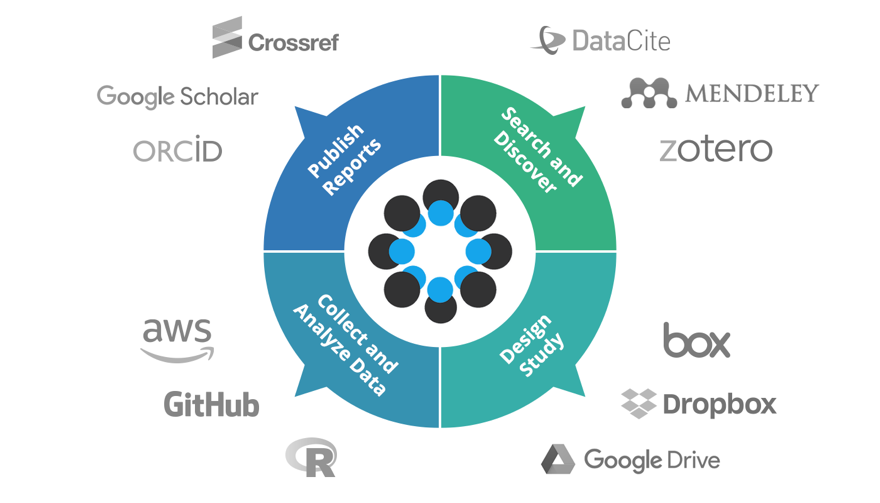
\includegraphics[width=0.28\textwidth]{images/osfframework}
\caption[Open Science Framework]{Open Science Framework}
\label{fig:openscienceframework}
\end{center}
\end{wrapfigure}
The \gls{ps} is the context of this research. \Gls{socialresponsbility} is important for this sector. To support \gls{socialresponsbility} this research and thesis are based on \gls{openscience}. \textcite{UNESCO2020} states that the idea behind Open Science is to allow scientific information, data and outputs to be more widely accessible (Open Access) and more reliably harnessed (Open Data) with the active engagement of all the stakeholders (Open to Society). The Center for Open Science\footnote{{\url{https://www.cos.io/}}} supports this way of research by supplying guidelines and a toolkit. For this research, the \gls{openscience} framework is used to support Open Access, Open Data and Open to Society. One of the tools in the framework is a reference model to select tools for the four main phases of research: Search and Discover, Design Study, Collect and Analyse Data, and Publish Reports, \cref{fig:openscienceframework}. See \cref{tab:openscienceframework} on how the \gls{openscience} framework is operationalised for this research. 
\begin{table}[H]
	\centering
	\resizebox{\textwidth}{!}{%
		\begin{tabular}{p{.25\linewidth}p{.75\linewidth}}
			\toprule
			\textbf{Open Science Framework} & \textbf{Operationalisation} \\
			\midrule
			 Open Science Framework & The Open Science Framework is used to define the processes and used tools. The framework will help in achieving replicability, precision, and reusability. \\%
			\bottomrule
		\end{tabular}
	}%
	\caption[Operationalisation of the Open Science Framework]{Operationalisation of the Open Science Framework}%
	\label{tab:openscienceframework}%
\end{table}

\subsection{Triangulation}
\label{sub:triangulation}
\Gls{triangulation} has its origins in geography. To know the position of a distant object, two checkpoints are needed. The mutual distance between the calibration points and the angles relative to the object make it possible to calculate the correct distance via triangulation\footnote{\url{https://www.britannica.com/science/triangulation-trigonometry}} \parencite[p.~88]{Mortelmans2018}. Following \textcite[p.~88]{Recker2012} \gls{triangulation} literally means doing more than just one thing \parencite[p.~88]{Recker2012}. According to \textcite[p.~110]{Recker2012} \gls{triangulation} means you are seeking convergence and corroboration of results from different methods and designs studying the same phenomenon. Through \gls{triangulation}, the researcher can gain a more nuanced picture of the situation and increase the reliability and validity of their findings \parencite[p.~88]{Recker2012}. \textcite[p.~88]{Recker2012} states that the use of \gls{triangulation} assists researchers in increasing the \gls{robustness} of results. Findings can be strengthened through the cross-validation achieved when different kinds and sources of data converge and are found to be congruent \parencite[p.~88]{Recker2012}. \textcite[p.~207]{Saunders2015} states that \gls{triangulation} involves using more than one source of data and method of collection to confirm the validity, credibility, and authenticity of research data, analysis and interpretation. \textcite[p.~207]{Saunders2015} also stresses that it is a necessity to use \textit{\gls{triangulation}} for a multi-method quantitative study, multi-method qualitative study or a mixed-methods study.

\textcite[p.~481]{Mortelmans2018} explains that in the qualitative research tradition, \gls{triangulation} has become the method of choice for increasing the credibility of results. It is stated by \textcite[p.~481]{Mortelmans2018} that there are four types of \gls{triangulation}. According to \textcite[p.~88]{Mortelmans2018} the first type is that of \textit{Data \Gls{triangulation}}. \textcite[p.~481]{Mortelmans2018} states that with \textit{Data \Gls{triangulation}}, different types of data are collected. The condition here is that the researcher stays within the qualitative paradigm \parencite[p.~481]{Mortelmans2018}. \textcite[p.~481]{Mortelmans2018} defines the second type \textit{Researcher \Gls{triangulation}}. To avoid case contamination, multiple researchers analyse the same data \parencite[p.~482]{Mortelmans2018}. Afterwards, the results are compared with each other, and it is examined where any differences come from \parencite[p.~482]{Mortelmans2018}. The third case is defined by \textcite[p.~481]{Mortelmans2018} as \textit{Theory \Gls{triangulation}}. \textcite[p.~482]{Mortelmans2018} explains that \textit{Theoretical \Gls{triangulation}} means triangulating the results from different theoretical angles. Looking at data from a different perspective often yields compelling \parencite[p.~482]{Mortelmans2018}. The last type of \gls{triangulation} is defined by \textcite[p.~481]{Mortelmans2018} as \textit{Methodological \Gls{triangulation}}. According to \textcite[p.~483]{Mortelmans2018} explains \textit{Methodological \Gls{triangulation}} as the combination of data collected by qualitative technique with data collected by quantitative means. However, \textcite[p.~483]{Mortelmans2018}\textit{Methodological \Gls{triangulation}} explains it does not necessarily mean that quantitative methods are applied in research. 
\begin{figure}[H]
	\centering
	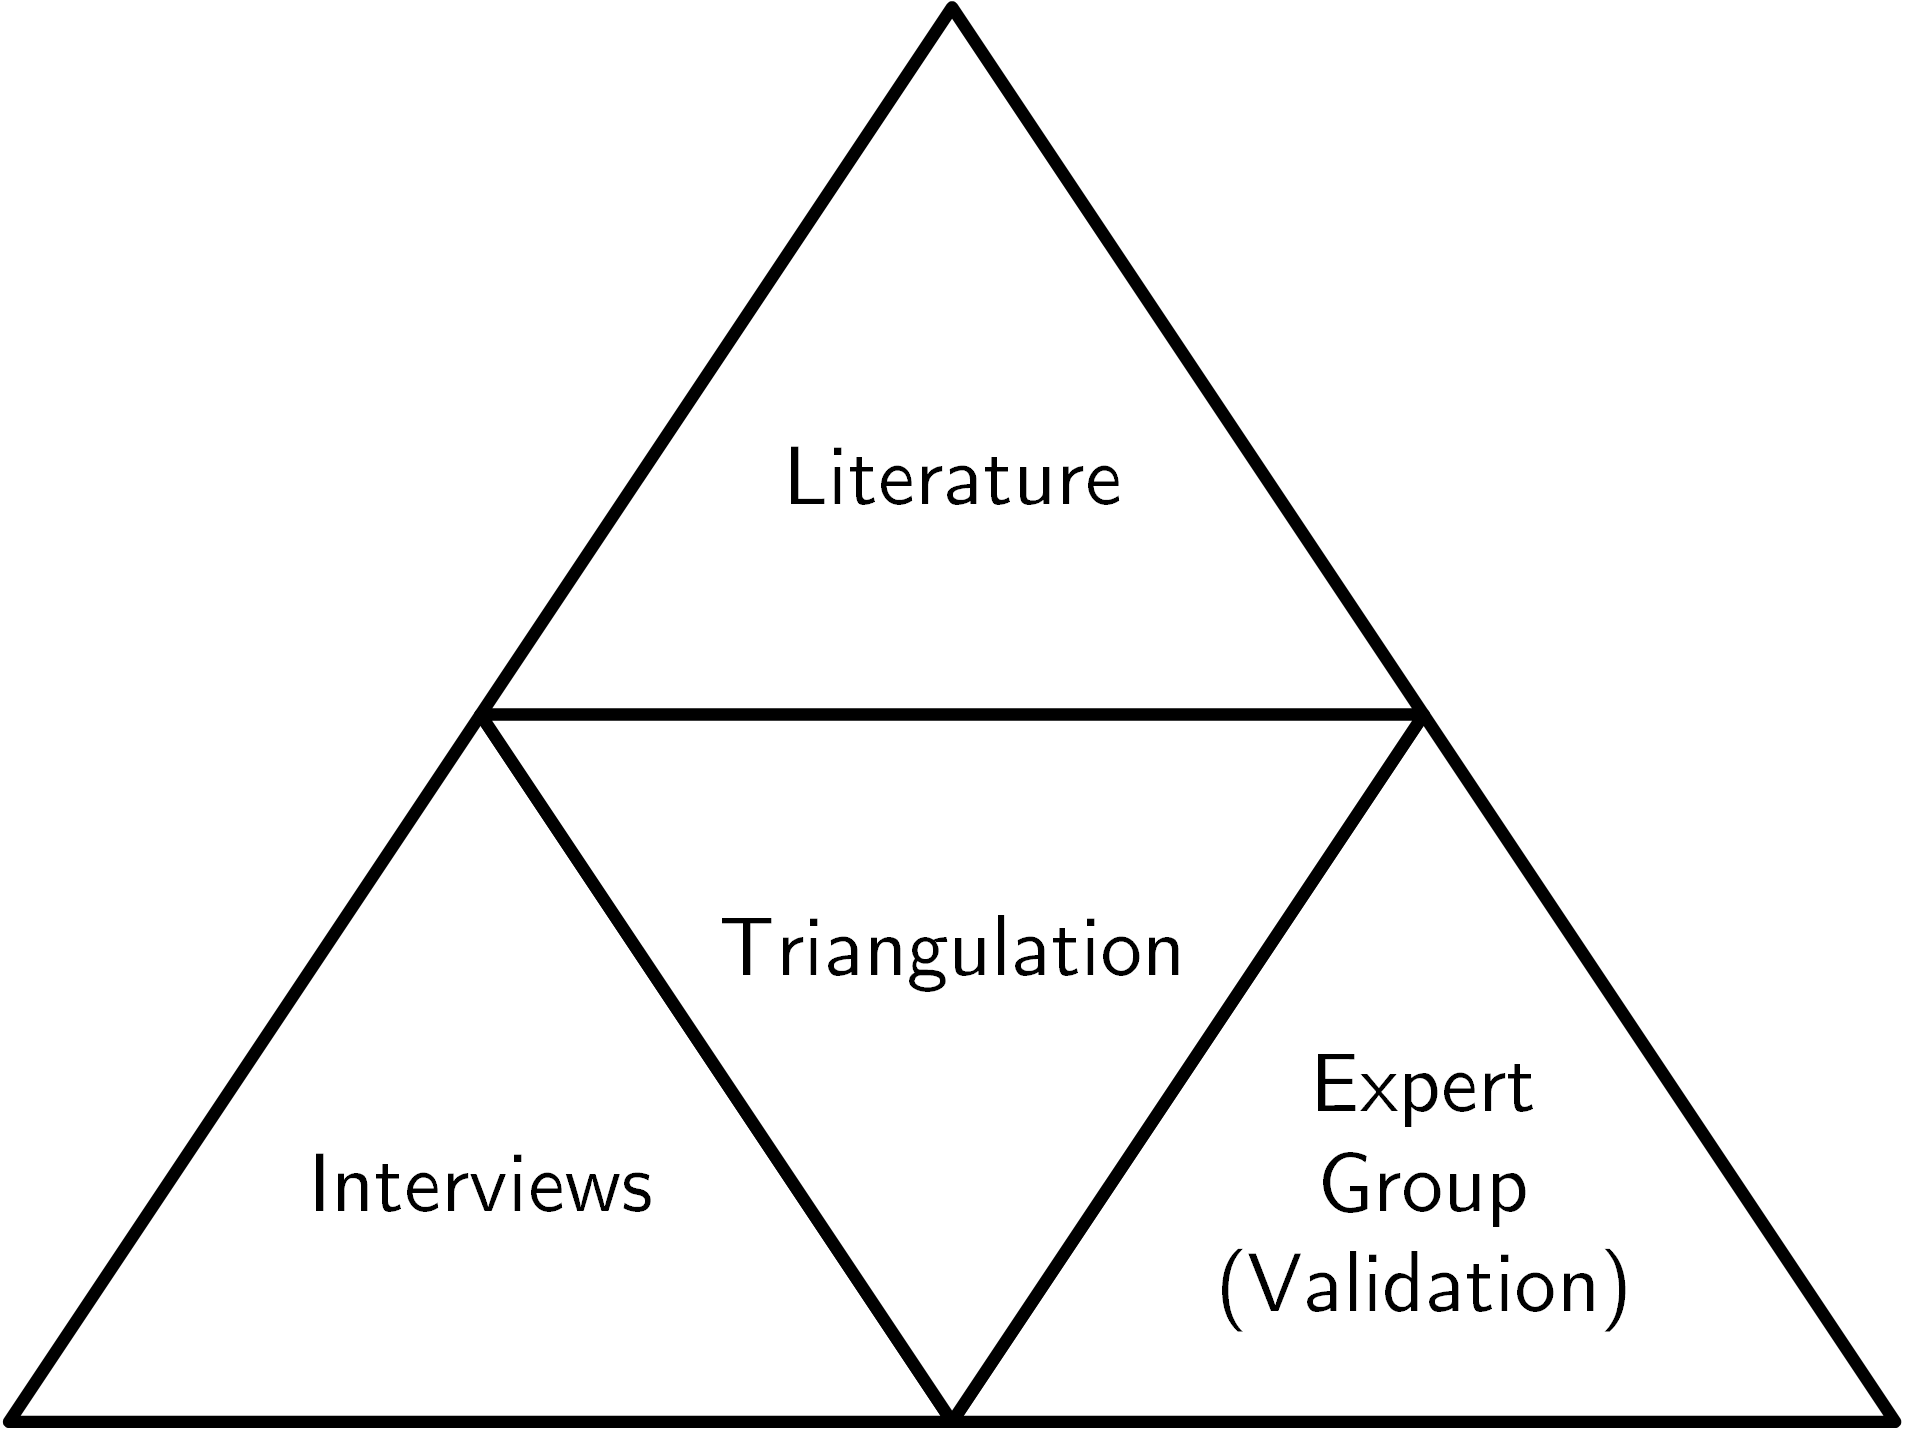
\includegraphics[width=0.5\linewidth]{images/triangulation}
	\caption[Operationalisation of Triangulation]{Operationalisation of Triangulation}
	\label{fig:triangulation}
\end{figure}
Triangulation is operationalised as Methodological Triangulation by using, as visualised by \cref{fig:triangulation}, literature study to abstract attributes, interviews with data analysis to validate attributes and an expert group with data analysis to validate attributes. 

\section{Research infrastructure and tooling}
\label{sec:researchinfraandtooling}
For selecting the suitable instruments for the research, the Open Science Framework\footnote{\url{https://www.cos.io/products/osf}} is used, see \cref{fig:openscienceframework}. The Open Science Framework proposes specific infrastructure and tools per stage. The transparency in the used infrastructure and tools increases the quality of the research by increasing replicability, findability, accessibility, interoperability, and reusability.
\subsection{Research execution}
\label{sub:tbresearchexecution}
For the execution of the research, Microsoft Excel\footnote{\url{https://www.microsoft.com/en-us/microsoft-365/excel}} is used for the administration of the literature research. For the administration of the literature research, the following headers are used: ID (for a unique ID per item), search terms used, scope, title, subtitle, author(s), year, type, Bib\LaTeX\ citation key, title relevance, abstract relevance, content relevance, found at, doi/isbn, url, date found, duplicate, date used, use for, and notes. Researchgate\footnote{\url{https://www.researchgate.net/}}, Web of Science\footnote{\url{https://app.webofknowledge.com/}}, Google Scholar\footnote{\url{https://scholar.google.com/}}, and Semantic Scholar\footnote{\url{https://www.semanticscholar.org/}} are the main sources for searching for literature. PaperPanda\footnote{\url{https://paperpanda.app/}} is used for hard to find literature. The literature administration is, together with the publicly available literature, stored in the repository of the master thesis\footnote{\url{https://github.com/JRBliekendaal/master-thesis/tree/main/literature}}. For non-public available literature, the administration contains the location where the literature is retrievable. All the literature is added to a bib\LaTeX\ file for future reference. For traceability the entries in the bib\LaTeX\ file contain the Unique ID in the notes field. JabRef is used to sort the references by using subgroups to support the workflow. The subgroups used are: ''evaluate, rejected, and used.'' Only the literature in the subgroup used are transferred to the bibliography file of the thesis. This prevents cluttering. For working as paperless as possible all the literature, where possible, is in pdf or in ebook format. For reading Acrobat Reader DC\footnote{\url{https://get.adobe.com/reader/}} is used for reading the PDF, and an Amazon Kindle Oasis\footnote{\url{https://www.amazon.com/dp/B07L5GJD99}} for eBooks. With the Amazon Kindle the highlight feature is used. This is not stored on GitHub since the highlights are under copyright of the author(s). For interviews Microsoft Teams is used with the transcript and session recording functionality. The transcript is full of sensitive information and is not publicly available. To make sure that the necessary information is available summaries are created and added to the thesis. The recordings are securely stored and are available upon request by the Antwerp Management School. The transcripts are used in QDA Minder Lite\footnote{\url{https://provalisresearch.com/products/qualitative-data-analysis-software/freeware/}} to label the interviews so that analysis can be done with Microsoft Excel. For the Expert Group, Meetingwizard\footnote{\url{https://www.meetingwizard.nl/}} is used for brainstorming, surveys and voting. The license for using Meeting Wizard is supplied by the Antwerp Management School. The output of the Meeting Wizard session is stored as a Microsoft Excel file in the repository of the thesis (anomysed).
\subsection{Research administration}
\label{sub:tbresearchadministration}
The research administration, which includes documentation containing privacy-sensitive information, like the name and contact information of the Expert Group participants, is stored on a non-public GitHub Repository\footnote{\url{https://github.com/JRBliekendaal/master-thesis-administration}}. The private GitHub Repository is also for staging thesis parts that still need to be anonymised. For taking notes Leuchtturm1917\footnote{\url{https://www.leuchtturm1917.us/notebook-classic.html}} Notebooks are used a mechanical pencil of Rotring\footnote{\url{https://www.rotring.com/pens-pencils/pencils/rotring-600-mechanical-pencil-1/SAP_1904443.html}}.
\subsection{Thesis creation}
\label{sub:tbresearchcreation}
I used my Apple MacBook Air M1 for creating the thesis. The thesis is created with the markup language \LaTeX\footnote{\url{https://www.latex-project.org/}}. The used typesetting environment is MacTex\footnote{\url{https://www.tug.org/mactex/}} with the document type of ''Report'' from KOMA-Script\footnote{\url{https://ctan.org/pkg/koma-script}}. TexStudio\footnote{\url{https://www.texstudio.org/}} is the used \LaTeX\ Editor. It supports syntax-highlighting, has an integrated viewer, reference checking and numerous wizards. For the creation and administration of references Bib\LaTeX\footnote{\url{https://ctan.org/pkg/biblatex/}} is used with the reference manager JabRef\footnote{\url{https://www.jabref.org/}} with the citation style of APA 7th Edition\footnote{\url{https://apastyle.apa.org/}} and with web browser integration. The files are stored on a personal Dropbox\footnote{\url{https://www.dropbox.com/}} that is used by GitHub Desktop\footnote{\url{https://desktop.github.com/}} to synchronise with a public GitHub repository\footnote{\url{https://github.com/JRBliekendaal/master-thesis}}. GitHub\footnote{\url{https://github.com/}} is used for source control but also for reviewing and discussing the topics with my (Co-)Promotor and the planning of the master thesis project. The thesis source files are copied to an Amazon S3 Blob\footnote{\url{https://aws.amazon.com/s3/}} for backup. The backup rotation is seven versions. Cloudberry Explorer Freeware for Amazon S3\footnote{\url{https://www.msp360.com/explorer/windows/amazon-s3.aspx}} is used for backup. Grammarly\footnote{\url{https://www.grammarly.com}}, with the paid subscription service, checks the thesis for spelling, grammar,  style, and plagiarism. The used goals for Grammarly are audience=knowledgeable, formality=formal, and domain=academic. Microsoft Visio Professional\footnote{\url{https://www.microsoft.com/en-ww/microsoft-365/visio/}} is used to create figures. The GitHub repository contains all the sources\footnote{\url{https://github.com/JRBliekendaal/master-thesis/tree/main/images/sources}}.
\subsection{Summary of used infrastructure and tooling}
The following tools are used to execute the research project:
\begin{table}[H]
	\begin{center}
		\resizebox{\textwidth}{!}{%
		\begin{tabular}{@{}llll@{}}
			\toprule
			\textbf{Search \& Discover} & \textbf{Design Study} & \textbf{Collect \& Analyse Data} & \textbf{Publish Reports}\\ \midrule
			Web of Science 	& bib\LaTeX  			& bib\LaTeX						& \LaTeX \\%
			ResearchGate   	& JabRef				& JabRef   						& TeXstudio \\%
			Google Scholar 	& Meetingwizard			& PaperPanda  					& ORCID \\%
			Semantic Scholar& Microsoft Excel 		& GitHub						& ResearchGate \\%
			doi.org			& Adobe Acrobat Reader	& Dropbox						& Zenodo \\%
			Microsoft Excel	& Amazon Kindle			& QDA Miner Lite				& Grammarly \\%
			    			& Microsoft Visio 		& Cloud Berry Explorer for S3 	&  \\%
			    			&						& Microsoft Excel				&	\\%
			\bottomrule
		\end{tabular}
		}%
		\caption{Used infrastructure \& tooling}
		\label{tab:usedinfrastructuretooling}
	\end{center}
\end{table}